\section{Ergänzungen zur Systemdokumentation}

\subsection{Fachklassendiagramm}
\label{subsec:fachklassendiagramm}

In Abbildung \ref{figure:fachklassen} ist eine Übersicht über die zentralen Fachklassen der Anwendung zu finden. Da JavaScript hier nicht als klassenorientierte Sprache verwendet wird, handelt es sich nicht um Klassen im engeren Sinn. Eine UML-Klasse wird hier für eine JavaScript-Funktion verwendet. Als Attribute werden lokale Variablen verwendet. Um Klassenmethoden umzusetzen, wurden die entsprechenden Funktionen dem Prototypen der Funktion hinzugefügt. Eine UML-Assoziation bedeutet, dass die \enquote{Klasse}, die eigentlich eine Funktion ist, eine andere \enquote{Klasse} in einer ihrer Methoden aufruft.

Durch das Diagramm wird ausgedrückt, wie sich die Fachklassen zueinander Verhalten. Die Controller ganz links greifen auf die Mustache-Views zu, die wiederum ihre Daten aus den Models beziehen. Der {\fontfamily{pcr}\selectfont ConflictDetector} wird unabhängig von den Fachklassen durch Input aus der Datenbank aufgerufen. Er ruft ggf. den {\fontfamily{pcr}\selectfont ConflictPresenter} auf, um Konflikte darzustellen, oder den {\fontfamily{pcr}\selectfont ConflictResolver}, um sie aufzulösen. Dafür benötigt letzterer auch Daten aus einer {\fontfamily{pcr}\selectfont NoteView} und der {\fontfamily{pcr}\selectfont NotesCollection}. Der {\fontfamily{pcr}\selectfont ConflictResolver} kann auch von einer {\fontfamily{pcr}\selectfont NotesView} aufgerufen werden, um einen Write-Konflikt darzustellen. 

\medskip
\begin{figure}[H] 
  \begin{center}
  \includegraphics[width=\textwidth]{grafik/Fachklassendiagramm} 
  % width=\textwidth,height=\textheight,keepaspectratio
  \end{center}
  \caption{Fachklassendiagramm}
  \label{figure:fachklassen}
\end{figure}





\subsection{Abstraktion der grundlegenden Datenbankoperationen}

\lstset{language=javascript}
\medskip 
\begin{lstlisting}[label=code:resources, caption=Auszug aus {\fontfamily{pcr}\selectfont /\_attachments/app/lib/resources.js}]
var Resources = function(app, couchapp) {
  this.helpers({
    new_object: function(kind, callback) {
      this.partial(template_file_for(kind, 'new'), callback);
    },
    \\ [...]
    
    load_object_view: function(kind, id, callback){
      var context = this;
      couchapp.db.openDoc(id, {
        success: function(doc) {
          var _prototype = eval(kind);
          var view_prototype = eval(kind + 'View');
          var view = new view_prototype(new _prototype(doc));
          if(doc) {            
            callback(view);            
          } else {
            context.flash = {message: kind + ' with ID "' + id + '" not found.', type: 'error'};
          }
        },
        error: function() {
          context.notFound();
        }
      });
    },

    \\ [...]
  });
};
\end{lstlisting}



\subsection{Einrückung von Zeilen im Outline}


\lstset{language=html}
\medskip 
\begin{lstlisting}[label=code:outline-indent, caption=Zeile mit einem Kindknoten]
<li class="edit-note" id="edit_note_2">
  <form class="edit-note" action="#/notes/2" method="put" accept-charset="utf-8">
    <span class="space">&nbsp;</span>
    <a class="image">&nbsp;</a>
    <textarea class="expanding" id="edit_text_2" name="text">Some text</textarea>
    <input type="submit" value="Save" style="display:none;"/>
  </form>

  <ul class="indent">
    <li class="edit-note" id="edit_note_2a">
      <form class="edit-note" action="#/notes/2a" method="put" accept-charset="utf-8">
        <span class="space">&nbsp;</span>
        <a class="image">&nbsp;</a>
        <textarea class="expanding" id="edit_text_2a" name="text">More text</textarea>
        <input type="submit" value="Save" style="display:none;"/>
      </form>
    </li>
  </ul>
</li>
\end{lstlisting}




\subsection{Rendern der Zeilen eines Outlines}

\lstset{language=javascript}
\medskip 
\begin{lstlisting}[label=code:rendernotes, caption=Auszug aus {\fontfamily{pcr}\selectfont /\_attachments/app/helpers/note\_element.js}]
renderNotes: function(context, notes, counter){
  if (notes.notes.length == 0) return;
  if (notes.notes.length == 1) {
    context.unbindSubmitOnBlurAndAutogrow();
    context.bindSubmitOnBlurAndAutogrow();
    $('#spinner').hide();
    context.i = 0;
  }
  if(typeof(context.i)=="undefined"){
    context.i = counter;
  } else {
    context.i = context.i-1;
  }
  var note_object = notes.findById(this.id());
  var child_object = note_object.firstChildNoteObject(notes.notes);
  var next_object = note_object.nextNoteObject(notes.notes);
  
  notes.notes = notes.notes.remove(note_object);
  
  if(typeof(child_object)!="undefined"){
    this.renderFollowingNote(context, child_object, function(child){
      child.renderNotes(context, notes);
    });
  } 
  if(typeof(next_object)!="undefined"){
    this.renderFollowingNote(context, next_object, function(next){
      next.renderNotes(context, notes);
    });
  }
  if(typeof(next_object)=="undefined" && typeof(child_object)=="undefined"){
    context.unbindSubmitOnBlurAndAutogrow();
    context.bindSubmitOnBlurAndAutogrow();
  }
},

renderFollowingNote: function(context, note_object, callback){
  var this_note = this;
  context.partial('app/templates/notes/edit.mustache', {_id: note_object._id, text: note_object.text}, function(html) {
    if(typeof note_object.parent_id != "undefined"){
      $(html).appendTo(this_note.note_target.closest('li')).wrap('<ul class="indent"></ul>');
      callback(this_note.firstChildNote());
    } else {
      $(html).insertAfter(this_note.note_target.closest('li'));
      callback(this_note.nextNote());        
    }
  });
}
\end{lstlisting}




\subsection{Überwachen der Datenbank auf Änderungen von Anderen}

\lstset{language=javascript}
\medskip 
\begin{lstlisting}[label=code:changesfeed, caption= {\fontfamily{pcr}\selectfont /\_attachments/app/helpers/replication\_helpers.js}]
checkForUpdates: function(couchapp){
  var context    = this;
  var source     = context.getLocationHash();
  var url        = config.HOST + '/' + config.DB + 
                   '/_changes?filter=doingnotes/changed&source=' + source;   
  
  if(context.getOutlineId()){ 
    $.getJSON(url, function(json){
      var since = json.last_seq;
      var xmlhttp = new XMLHttpRequest();
      xmlhttp.onreadystatechange=function() {
        if(xmlhttp.readyState == 3){
          if(xmlhttp.responseText.match(/changes/)){
            var lines = xmlhttp.responseText.split("\n");
            if(lines[lines.length-2].length != 0){ 
              lines = lines.remove("");
              $.each(lines, function(i, line){
                context.parseLineAndShowChangesWarning(context, couchapp, line, lines);
              });
            }
          }
          if(xmlhttp.responseText.match(/last_seq/)){
            Sammy.log('Timeout in checkForUpdates:', xmlhttp.responseText)
          }
        }
      }
      xmlhttp.open("GET", url+ '&feed=continuous&heartbeat=5000&since=' +since, true);
      xmlhttp.send(null);
    });
  }
}
\end{lstlisting}








\subsection{Patch für den CouchDB Changes-Filter}
\label{subsec:changes-patch}



Die Funktion {\fontfamily{pcr}\selectfont make\_filter\_fun} erzeugt eine Funktion, die für jede Zeile im Changes-Feed das entsprechende Dokument lädt. Die angegebene Filterfunktion entscheidet anhand der JSON-Repräsentation des Dokuments, ob die Zeile in der Rückgabe des Changes-Feeds enthalten sein soll. Das {\fontfamily{pcr}\selectfont \_conflicts}-Array wurde in Zeile \ref{lst:addtopatch} dem JSON-Objekt hinzugefügt, so dass auch auf dieses von einer Filterfunktion berücksichtigt werden kann.



\lstset{language=erlang}
\medskip
\begin{lstlisting}[label=code:changes-patch,caption=Die Funktion {\fontfamily{pcr}\selectfont make\_filter\_fun},escapeinside={@}{@}]
make_filter_fun(Req, Db) ->
    Filter = couch_httpd:qs_value(Req, "filter", ""),
    case [list_to_binary(couch_httpd:unquote(Part))
            || Part <- string:tokens(Filter, "/")] of
    [] ->
        fun(DocInfos) ->
            [{[{rev, couch_doc:rev_to_str(Rev)}]} ||
                #doc_info{revs=[#rev_info{rev=Rev}|_]} <- DocInfos]
        end;
    [DName, FName] ->
        DesignId = <<"_design/", DName/binary>>,
        DDoc = couch_httpd_db:couch_doc_open(Db, DesignId, nil, []),
        #doc{body={Props}} = DDoc,
        couch_util:get_nested_json_value({Props}, [<<"filters">>, FName]),
        fun(DocInfos) ->
            Docs = [Doc || {ok, Doc} <- [
                @\label{lst:addtopatch}@{ok, Doc} = couch_db:open_doc(Db, DInfo, [deleted, conflicts])
                || DInfo <- DocInfos]],
            {ok, Passes} = couch_query_servers:filter_docs(Req, Db, DDoc, FName, Docs),
            [{[{rev, couch_doc:rev_to_str(Rev)}]}
                || #doc_info{revs=[#rev_info{rev=Rev}|_]} <- DocInfos, 
                Pass <- Passes, Pass == true]
        end;
    _Else ->
        throw({bad_request, 
            "filter parameter must be of the form `designname/filtername`"})
    end.  
\end{lstlisting}


Für den Test wurde ein Designdokument in die Testdatenbank eingefügt, das eine List-Funktion enthält, die alle Dokumente mit Konflikten ausgibt.

\lstset{language=javascript}
\medskip
\begin{lstlisting}[label=code:changes-patch-test,caption=Test für die Funktion in Listing \ref{code:changes-patch-test}]
var ddoc = {
  _id : "_design/changes_filter",
  "filters" : {
    "conflicted" : "function(doc, req) { return (doc._conflicts);}",
  }
}

var id = db.save({'food' : 'pizza'}).id;
db.bulkSave([{_id: id, 'food' : 'pasta'}], {all_or_nothing:true});

req = CouchDB.request("GET", "/test_suite_db/_changes?filter=changes_filter/conflicted");
resp = JSON.parse(req.responseText);
T(resp.results.length == 1);
\end{lstlisting}





\subsection{HTML-Datei zum Ausführen der Unit Tests}


\lstset{language=html}
\medskip 
\begin{lstlisting}[label=code:jspec-index,caption={\fontfamily{pcr}\selectfont /\_attachments/spec/index.html}]
<html>
  <head>
    <link rel="stylesheet" href="jspec/jspec.css" type="text/css"/>
    <script src="../../vendor/jquery/_attachments/jquery.js"></script>
    <script src="jspec/jspec.js"></script>
    <script src="jspec/jspec.jquery.js"></script>
    <script src="jspec/jspec.xhr.js"></script>
    <script src="../app/lib/lib.js"></script>
    <script src="../app/lib/resources.js"></script>
    <script src="../config/config.js"></script>
    <script src="../app/helpers/key_events.js"></script>
    <script src="../app/helpers/note_element.js"></script>
    <script src="../app/helpers/outline_helpers.js"></script>
    <script src="../app/models/note.js"></script>
    <script src="../app/models/outline.js"></script>
    <script src="../app/models/note_collection.js"></script>
    <script>
      function runSuites() {
        JSpec
        .exec('note_element_spec.js')
        .exec('inserting_note_element_spec.js')
        .exec('indenting_note_element_spec.js')
        .exec('unindenting_note_element_spec.js')
        .exec('focusing_note_element_spec.js')
        .exec('rendering_note_element_spec.js')
        .exec('outline_helpers_spec.js')
        .exec('outline_spec.js')
        .exec('note_spec.js')
        .exec('note_collection_spec.js')
        .exec('resources_spec.js')
        .exec('lib_spec.js')
        .exec('conflict_spec.js')
        .run({failuresOnly: true, fixturePath: 'fixtures'})
        .report();
      }
    </script>
  </head>
	<body class="jspec" onLoad="runSuites();">
		<div id="jspec"></div>
	</body>
</html>
\end{lstlisting}










\subsection{Testsuite für die CouchDB JavaScript HTTP API}
\label{subsec:httpapi}

\subsubsection{Auszug aus der CouchDB JavaScript HTTP API}

\lstset{language=javascript}
\medskip 
\begin{lstlisting}[label=code:httpapi, caption=Auszug aus {\fontfamily{pcr}\selectfont /share/www/script/jquery.couch.js}]
(function($) {
  \\ [...]
  $.extend($.couch, {
    \\ [...]
    db: function(name) {
      \\ [...]
      return {
        \\ [...]
        removeDoc: function(doc, options) {
          ajax({
              type: "DELETE",
              url: this.uri +
                   encodeDocId(doc._id) +
                   encodeOptions({rev: doc._rev})
            },
            options,
            "The document could not be deleted"
          );
        }
        \\ [...]
      };
    }
    \\ [...]
  });
})(jQuery);
\end{lstlisting}


\subsubsection{Der Test f\"ur Listing \ref{code:httpapi}}
\label{subsec:testsuite-jspec-code}

\medskip
\begin{lstlisting}[label=code:httpapitest, breaklines=true, caption=Auszug aus {\fontfamily{pcr}\selectfont /share/www/spec/jquery\_couch\_3\_spec.js}]
describe 'jQuery couchdb db'
  \\ [...]
  
  before_each
    db = $.couch.db('spec_db');
    db.create();
  end
  
  after_each
    db.drop();
  end

  describe 'removeDoc'
    before_each
      doc = {"Name" : "Louanne Katraine", "Callsign" : "Kat", "_id" : "345"};
      saved_doc = {};
      db.saveDoc(doc, {
        success: function(resp){
          saved_doc = resp;
        },
        error: function(status, error, reason){errorCallback(status, error, reason)}
      });
    end
    
    it 'should result in a deleted document'
      db.removeDoc({_id : "345", _rev : saved_doc.rev}, {
        success: function(resp){
          db.openDoc("345", {
            error: function(status, error, reason){
              status.should.eql 404
              error.should.eql "not_found"
              reason.should.eql "deleted"
            },
            success: function(resp){successCallback(resp)}
          });
        },
        error: function(status, error, reason){errorCallback(status, error, reason)}
      });
    end
  
    it 'should return ok true, the ID and the revision of the deleted document'
      db.removeDoc({_id : "345", _rev : saved_doc.rev}, {
        success: function(resp){
          resp.ok.should.be_true
          resp.id.should.eql "345"
          resp.rev.should.be_a String
          resp.rev.length.should.be_at_least 30
        },
        error: function(status, error, reason){errorCallback(status, error, reason)}
      });
    end
      
    it 'should record the revision in the deleted document'
      db.removeDoc({_id : "345", _rev : saved_doc.rev}, {
        success: function(resp){
          db.openDoc("345", {
            rev: resp.rev,
            success: function(resp2){
              resp2._rev.should.eql resp.rev
              resp2._id.should.eql resp.id
              resp2._deleted.should.be_true
            },
            error: function(status, err, rsn){errorCallback(status, err, rsn)}
          });
        },
        error: function(status, error, reason){errorCallback(status, error, reason)}
      });
    end
    
    it 'should alert with an error message prefix'
      db.removeDoc({_id: "asdf"});
      alert_msg.should.match /The document could not be deleted/
    end
  end

  \\ [...]
end
\end{lstlisting}







\newpage
\subsection{Screenshots der AWS Management Console}
\label{subsec:aws}

\begin{figure}[H] 
  \begin{center}
    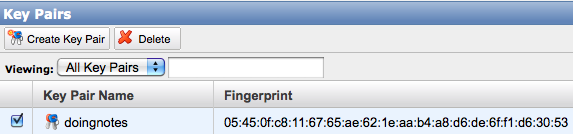
\includegraphics[width=\textwidth]{grafik/aws-key-pair} 
  \end{center}
  \caption{AWS: Schlüsselpaar für die Authentifizierung}
  \label{fig:aws-key}
\end{figure}

\begin{figure}[H] 
  \begin{center}
    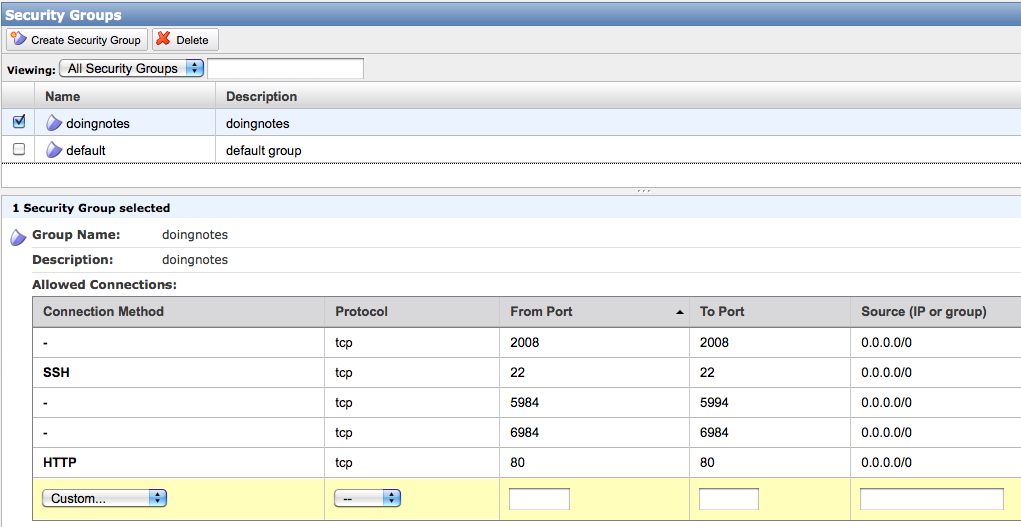
\includegraphics[width=\textwidth]{grafik/aws-security-group} 
  \end{center}
  \caption{AWS: Freigeben der Ports über die Security Group}
  \label{fig:aws-group}
\end{figure}

\begin{figure}[H] 
  \begin{center}
    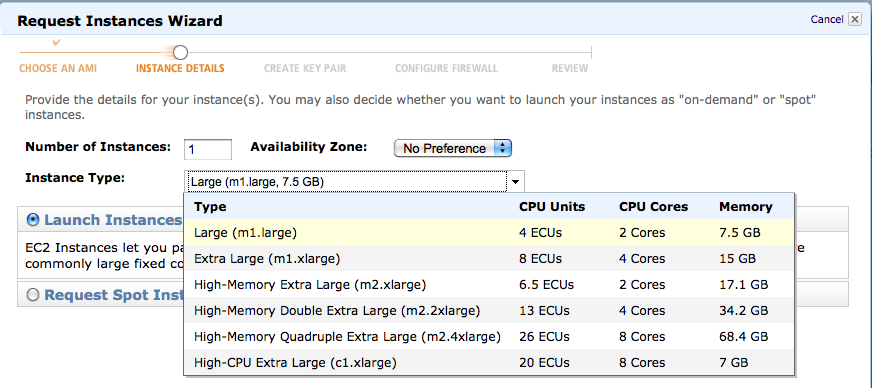
\includegraphics[width=\textwidth]{grafik/aws-select-size} 
  \end{center}
  \caption{AWS: Auswahl der Kapazitäten der Instanz}
  \label{fig:aws-size}
\end{figure}

\begin{figure}[H] 
  \begin{center}
    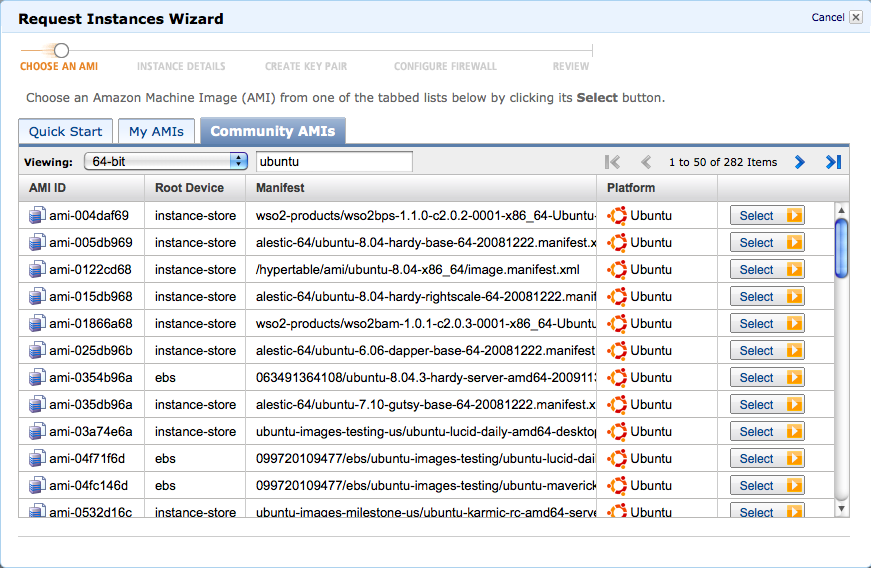
\includegraphics[width=\textwidth]{grafik/aws-select-AMI} 
  \end{center}
  \caption{AWS: Auswahl des Amazon Machine Images}
  \label{fig:aws-ami}
\end{figure}

\begin{figure}[H] 
  \begin{center}
    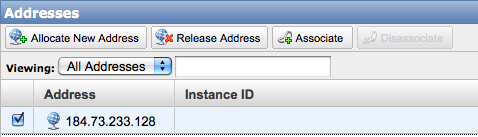
\includegraphics[width=\textwidth]{grafik/aws-ip} 
  \end{center}
  \caption{AWS: Einrichten einer Elastic IP}
  \label{fig:aws-ip}
\end{figure}

\begin{figure}[H] 
  \begin{center}
    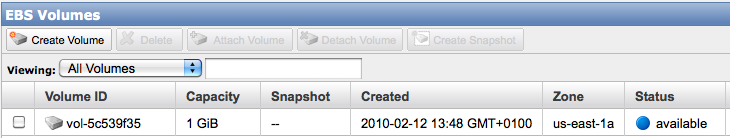
\includegraphics[width=\textwidth]{grafik/aws-ebs-volume} 
  \end{center}
  \caption{AWS: Einrichten eines EBS Volumes}
  \label{fig:aws-ebs}
\end{figure}


\begin{figure}[H] 
  \begin{center}
    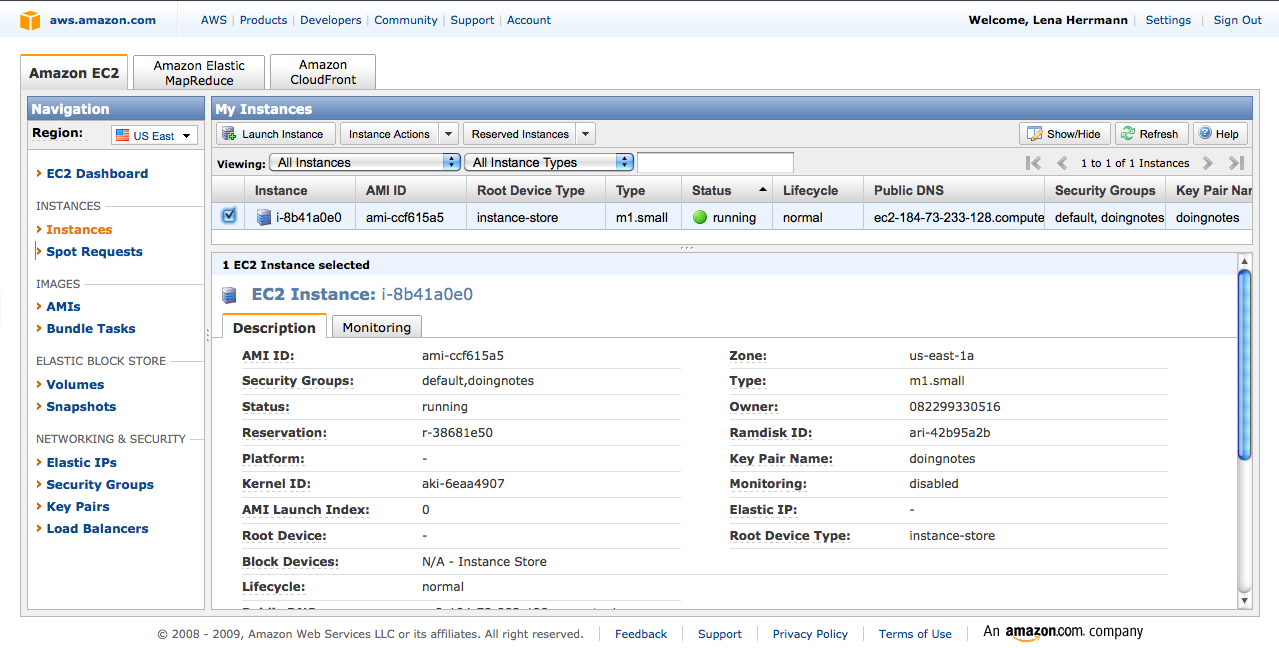
\includegraphics[width=\textwidth]{grafik/aws-ec2-management-console} 
  \end{center}
  \caption{AWS: Die laufende EC2-Instanz}
  \label{fig:aws-console}
\end{figure}

